% cd /storage/emulated/0/Documents/documents/latex/1920/Grade-10/1st/area-of-sectors-and-segments-of-a-circle && pdflatex ps-area-of-sectors-and-segments-of-a-circle.tex && termux-open ps-area-of-sectors-and-segments-of-a-circle.pdf

% cd /storage/emulated/0/Documents/documents/latex/1920/Grade-10/1st/area-of-sectors-and-segments-of-a-circle && clean-tex ps-area-of-sectors-and-segments-of-a-circle-input1.tex


% cd /storage/emulated/0/Documents/documents/latex/1920/Grade-10/1st/area-of-sectors-and-segments-of-a-circle && convert -density 600 ps-area-of-sectors-and-segments-of-a-circle.pdf -crop 2200x1700 -quality 100 -verbose ps-area-of-sectors-and-segments-of-a-circle%02d.png

%2480.5x3508 portrait 2x2 2550x3300
%3508x2480.5 landscape 2x2 3300x2550 
%1653.7x2338.7 portrait 3x3 1700x2200
%landscape 3x3 2200x1700

% cd /storage/emulated/0/Documents/documents/latex/1819/grade10/visual/4th/area-of-sectors-and-segments-of-a-circle && while inotifywait -e close_write ps-area-of-sectors-and-segments-of-a-circle*.tex; do touch /storage/emulated/0/Android/data/com.termux/files/launch-termux.txt && printf '1' > /storage/emulated/0/Android/data/com.termux/files/launch-termux.txt && pdflatex ps-area-of-sectors-and-segments-of-a-circle.tex && termux-open ps-area-of-sectors-and-segments-of-a-circle.pdf; done

% cd /host-rootfs/storage/emulated/0/Documents/documents/latex/1819/grade10/visual/4th/area-of-sectors-and-segments-of-a-circle && while inotifywait -e close_write ps-area-of-sectors-and-segments-of-a-circle*.tex; do pdflatex ps-area-of-sectors-and-segments-of-a-circle.tex  && printf "/storage/emulated/0/Documents/documents/latex/1819/grade10/visual/4th/area-of-sectors-and-segments-of-a-circle/ps-area-of-sectors-and-segments-of-a-circle.pdf" > /host-rootfs/storage/emulated/0/GNURoot/home/Scripts/file-to-launch.txt; done


\documentclass[10pt]{article}
\usepackage[letterpaper, landscape, right=0.25in, left=0.25in, top=0.25in, bottom=0.25in]{geometry}
\usepackage{xcolor}
\usepackage{anyfontsize}
\usepackage{enumitem}
\usepackage{multicol}
\usepackage{amsmath}
%\usepackage{amsfonts,dsfont}% for \mathds 
\usepackage{tabularx} 
\usepackage{gensymb}
\usepackage{multirow}
\usepackage{graphicx, tipa}
\usepackage{tikz}
\usetikzlibrary{angles,quotes}
\usepackage{pgfplots} 
\usetikzlibrary{calc}
\pgfplotsset{compat=newest}
\usetikzlibrary{arrows.meta}
\usetikzlibrary{intersections}
\usetikzlibrary{decorations.pathreplacing}
\usepackage{flafter}
\usepackage{amsmath,amssymb,cancel,units}
\usepackage{microtype} % nicer output 
\usepackage{hfoldsty} % nicer output 
\usepackage{fixltx2e} 
\usepackage{mathptmx}
%\usepackage{booktabs}
\usepackage{numprint}
\usepackage[utf8]{inputenc} 
\usepackage[T1]{fontenc}
%\usepackage{siunitx} 
%\sisetup{detect-all}


\def\radA{3.6cm}

\def\radB{3.6cm}

%\def\thirdrad{8cm}

\pagenumbering{gobble}
%\linespread{0.9}
\newcommand{\vspce}{\vspace{0.75ex}}
\newcommand{\hspce}{\hspace{0.5em}}
\newcommand{\blank}{\underline{\hspace{2em}}}%{\rule{1em}{0.15ex}}
\newcommand{\arc}[1]{{% 
\setbox9=\hbox{#1}% 
\ooalign{\resizebox{\wd9}{\height}{\texttoptiebar{\phantom{A}}}\cr#1}}}

\newcolumntype{C}{ >{\centering\arraybackslash} X}




\begin{document}
\boldmath
{\fontsize{36}{40}\fontfamily{pnc}\selectfont {

\def\curdir{/storage/emulated/0/Documents/documents/latex/1920/Grade-10/2nd/area-of-sectors-and-segments-of-a-circle/fig-a}

\def\radA{1.2cm}

\textbf{Practice Exercises}

\vspce

Find the area of each shaded region/s in each figure.  Express your answer in terms of $\pi$. 
\begin{center}
\vspace*{-2ex}
\scalebox{1}{
\noindent\begin{minipage}{\textwidth}
{\begin{tabularx}{\textwidth}{XX}
1. 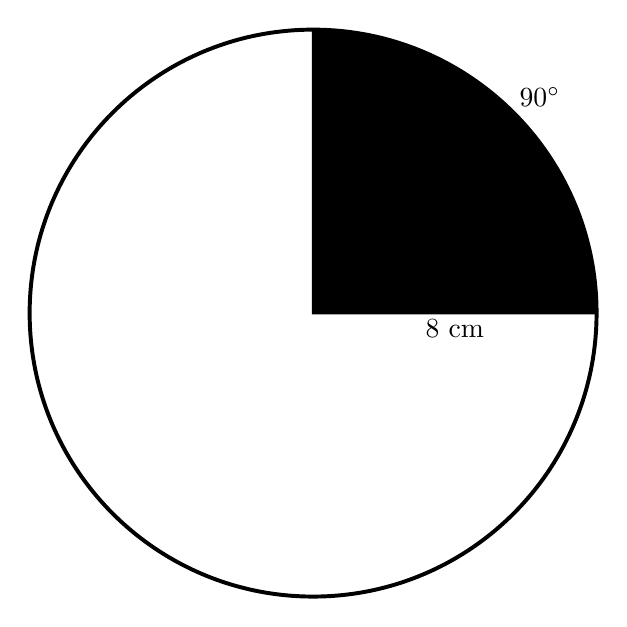
\begin{tikzpicture}[baseline = (current bounding box.west)]


\node[draw, circle, minimum size=2*\radA, inner sep=0pt, line width=0.5mm, outer sep=0] (circ) at (0,0) {};

\node[anchor=north, inner sep=2pt, rotate=0] (8cm.label) at ($(circ.center)!0.5!(0:\radA)$) {$ \text{8 cm}$};

\node[anchor=south west, inner sep=2pt, rotate=0] (90.label) at ($(circ.center)+(45:\radA)$) {$ 90 \degree $};

\filldraw[fill=\figurefill, line width=0.3mm]  (0:\radA) arc (0:90:\radA) -- (circ.center) -- cycle;

\end{tikzpicture} 
 & 5. 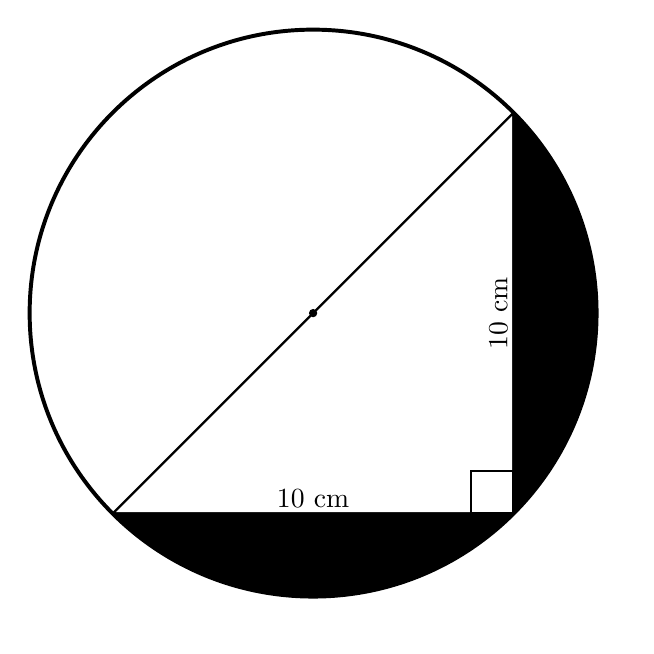
\begin{tikzpicture}[dot/.style={circle, fill=black, inner sep=0pt, outer sep=0pt, minimum size=3pt}, baseline = (current bounding box.west)]



\node[draw, circle, minimum size=2*\radA, inner sep=0pt, line width=0.5mm, outer sep=0] (circ) at (0,0) {};

\node[dot] (circ.dot)  at (circ) {}; 

\coordinate (a) at ($(circ) + (45:\radA)$); 

\coordinate (b) at ($(circ) - (45:\radA)$); 

\coordinate (c) at ($(circ) + (-45:\radA)$); 

\draw[line width=0.3mm] (a) -- (b) (b) -- (c) (c) -- (a) ;

\node[anchor=south, inner sep=2pt] (10cm1-label) at ($(b)!0.5!(c)$) {$ \text{10 cm}$};  

\filldraw[fill=\figurefill, line width=0.3mm]  (45:\radA) arc (45:-45:\radA) -- cycle;

\filldraw[fill=\figurefill, line width=0.3mm]  (-45:\radA) arc (-45:-135:\radA) -- cycle;

\node[anchor=south, inner sep=2pt, rotate=90] (10cm2-label) at ($(a)!0.5!(c)$) {$ \text{10 cm}$};  

\begin{scope} [rotate=90]
\draw[line width=0.3mm] (c) rectangle ++(0.15*\radA,0.15*\radA) node[transform shape]{};
\end{scope} 

\end{tikzpicture}  
 \\
2. 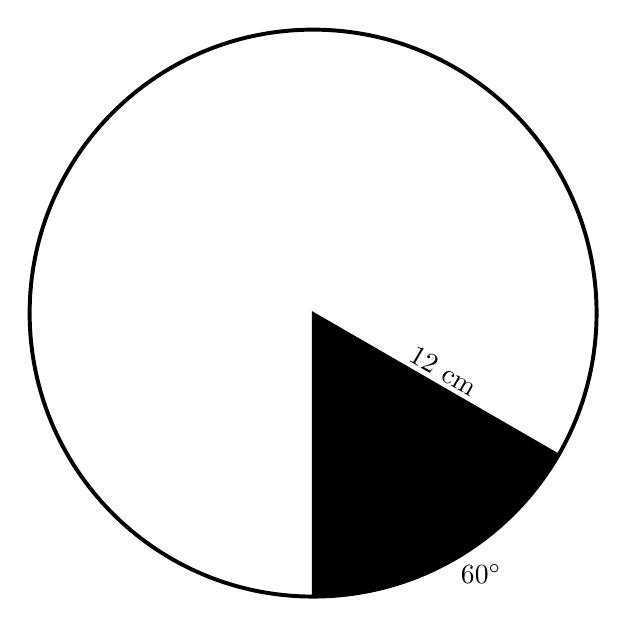
\begin{tikzpicture}[baseline = (current bounding box.west)]



\node[draw, circle, minimum size=2*\radA, inner sep=0pt, line width=0.5mm, outer sep=0] (circ) at (0,0) {};

\node[anchor=south, inner sep=2pt, rotate=-30] (12cm.label) at ($(circ.center)!0.5!(-30:\radA)$) {$ \text{12 cm}$};

\node[anchor=north west, inner sep=2pt, rotate=0] (60.label) at ($(circ.center)+(-60:\radA+0pt)$) {$ 60 \degree $};

\filldraw[fill=\figurefill, line width=0.3mm]  (-30:\radA) arc (-30:-90:\radA) -- (circ.center) -- cycle;

\end{tikzpicture} 

 & 6. 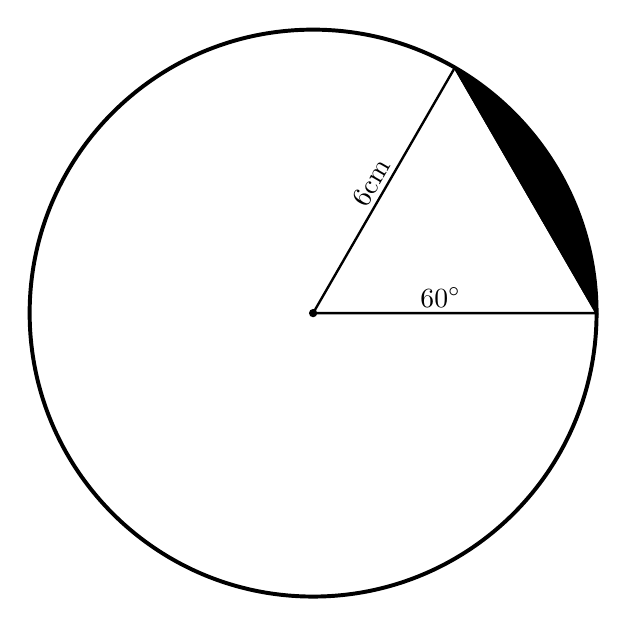
\begin{tikzpicture}[dot/.style={circle, fill=black, inner sep=0pt, outer sep=0pt, minimum size=3pt}, baseline = (current bounding box.west)]

\node[draw, circle, minimum size=2*\radA, inner sep=0pt, line width=0.5mm, outer sep=0] (circ) at (0,0) {};

\node[dot] (circ.dot)  at (circ) {}; 

\coordinate (a) at ($(circ) + (60:\radA)$); 

\coordinate (n) at ($(circ) + (0:\radA)$); 

\draw[line width=0.3mm] (a) -- (circ.center) -- (n) -- cycle;

\filldraw[fill=\figurefill, line width=0.3mm]  (0:\radA) arc (0:60:\radA) -- cycle;

\node[anchor=south, inner sep=2pt, rotate=60] (6cm1.label) at ($(circ.center)!0.5!(a)$) {$\text{6cm}$};

\node[anchor=south, inner sep=2pt, rotate=0] (60.label) at ($(circ.center)!0.45!(n)$) {$ 60 \degree $};

\end{tikzpicture}  
 \\
3. 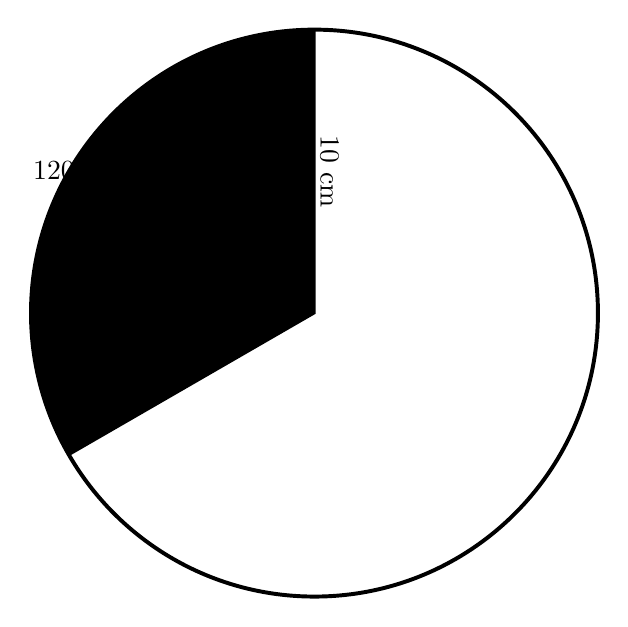
\begin{tikzpicture}[baseline = (current bounding box.west)]



\node[draw, circle, minimum size=2*\radA, inner sep=0pt, line width=0.5mm, outer sep=0] (circ) at (0,0) {};

\node[anchor=south, inner sep=2pt, rotate=-90] (10cm.label) at ($(circ.center)!0.5!(90:\radA)$) {$ \text{10 cm}$};

\node[anchor=south east, inner sep=2pt, rotate=0] (120.label) at ($(circ.center)+(150:0.9*\radA)$) {$ 120 \degree $};

\filldraw[fill=\figurefill, line width=0.3mm]  (90:\radA) arc (90:210:\radA) -- (circ.center) -- cycle;

\end{tikzpicture} 

 & 7. 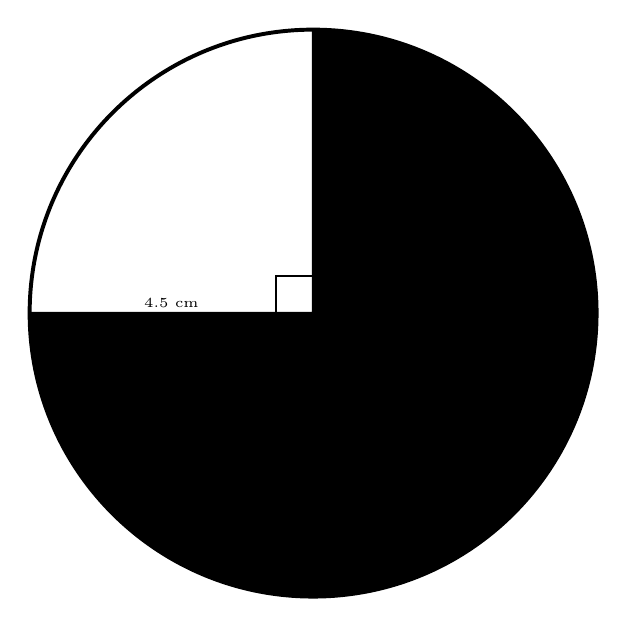
\begin{tikzpicture}[dot/.style={circle, fill=black, inner sep=0pt, outer sep=0pt, minimum size=0pt}, baseline = (current bounding box.west)]

\node[draw, circle, minimum size=2*\radA, inner sep=0pt, line width=0.5mm, outer sep=0] (circ) at (0,0) {};

\node[dot] (circ.dot)  at (circ) {}; 

\coordinate (a) at ($(circ) + (180:\radA)$); 

\coordinate (t) at ($(circ) + (90:\radA)$); 

\draw[line width=0.3mm] (a) -- (circ.center) -- (t) ;

\node[anchor=south, inner sep=2pt, rotate=0] (4.5cm-label) at ($(a)!0.5!(circ.center)$) {\tiny $ \text{4.5 cm} $};  

\filldraw[fill=\figurefill, line width=0.3mm]  (90:\radA) arc (90:-180:\radA) -- (circ.center) -- cycle;

\begin{scope} [rotate=90]
\draw[line width=0.3mm] (circ.center) rectangle ++(0.13*\radA,0.13*\radA) node[transform shape]{};
\end{scope} 

\end{tikzpicture}  
 \\
4. 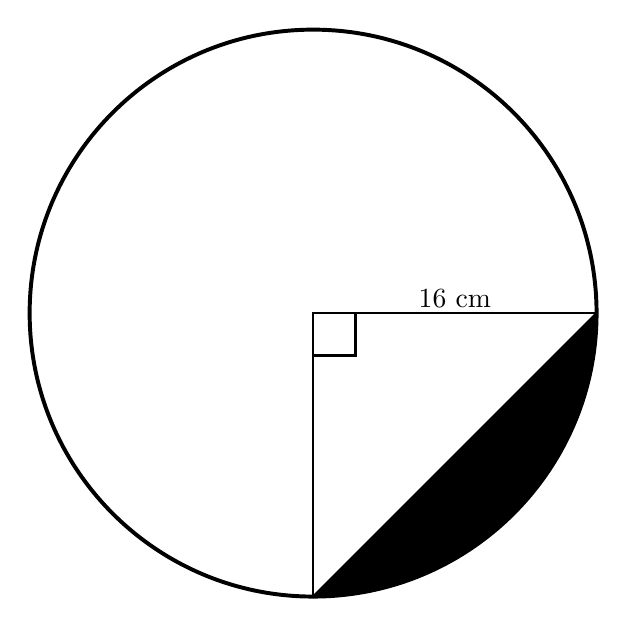
\begin{tikzpicture}[baseline = (current bounding box.west)]



\node[draw, circle, minimum size=2*\radA, inner sep=0pt, line width=0.5mm, outer sep=0] (circ) at (0,0) {};

\node[anchor=south, inner sep=2pt, rotate=0] (16cm.label) at ($(circ.center)!0.5!(0:\radA)$) {$ \text{16 cm}$};

\filldraw[fill=\figurefill, line width=0.3mm]  (0:\radA) arc (0:-90:\radA) -- cycle;

\draw[line width=0.3mm]  (0:\radA) -- (circ.center) -- (-90:\radA);

\begin{scope} [rotate=-90]
\draw[line width=0.3mm] (circ.center) rectangle ++(0.15*\radA,0.15*\radA) node[transform shape]{};
\end{scope} 

\end{tikzpicture} 
 & 8. 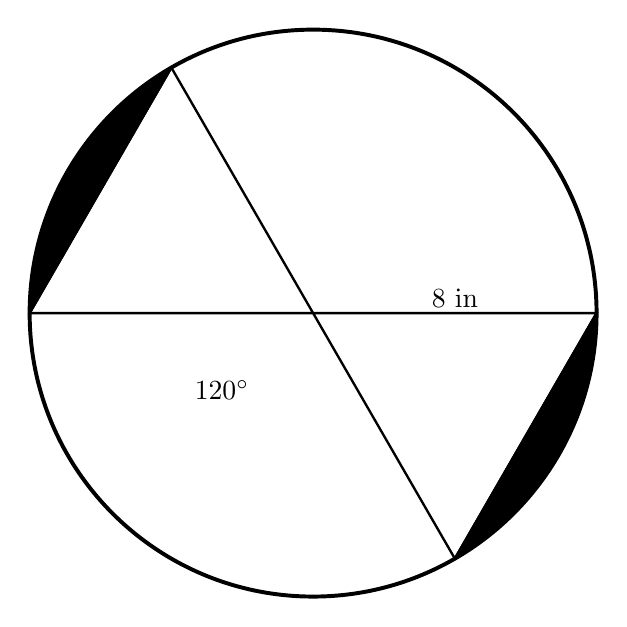
\begin{tikzpicture}[baseline = (current bounding box.west)]

\node[draw, circle, minimum size=2*\radA, inner sep=0pt, line width=0.5mm, outer sep=0] (circ) at (0,0) {};

\node[anchor=south, inner sep=2pt, rotate=0] (8in.label) at ($(circ.center)!0.5!(0:\radA)$) {$ \text{8 in}$};

\filldraw[fill=\figurefill, line width=0.3mm]  (0:\radA) arc (0:-60:\radA) -- cycle;

\filldraw[fill=\figurefill, line width=0.3mm]  (180:\radA) arc (180:120:\radA) -- cycle;

\node[rotate=0] (120-label) at ($(circ.center)+(220:0.42*\radA)$) {$ 120\degree $}; 

\draw[line width=0.3mm] (0:\radA) -- (180:\radA) -- (120:\radA) -- (-60:\radA) -- cycle;

\end{tikzpicture} 

 \\
\end{tabularx}}
\end{minipage}}
\end{center} 
  

%}} 

%\newpage

%{\fontsize{38}{40}\fontfamily{pnc}\selectfont {

\input{ps-area-of-sectors-and-segments-of-a-circle-input2}
}}
\newpage

{\fontsize{36}{40}\fontfamily{pnc}\selectfont {
\def\curdir{/storage/emulated/0/Documents/documents/latex/1920/Grade-10/2nd/area-of-sectors-and-segments-of-a-circle/fig-b}

\def\radB{1.7cm}

\textbf{Problem Set}

\vspce

Find the area of each shaded region/s in each figure.  Express your answer in terms of $\pi$. 
\begin{center}
\vspace*{-2ex}
\scalebox{1}{
\noindent\begin{minipage}{\textwidth}
{\begin{tabularx}{\textwidth}{XX}
1. 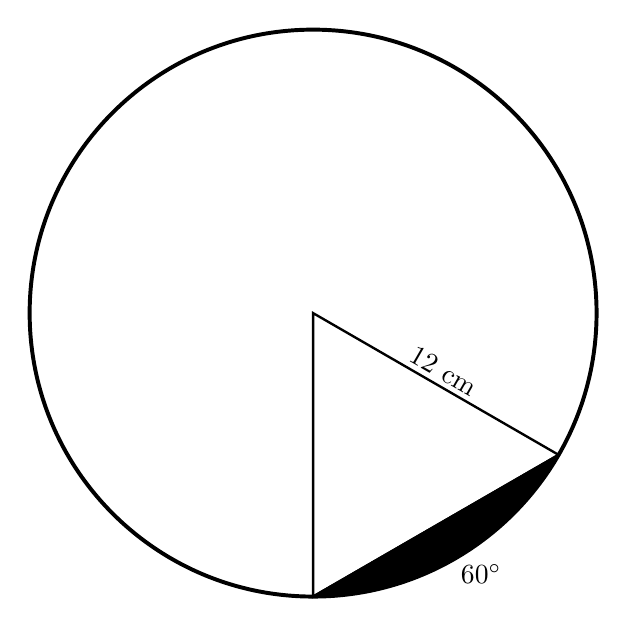
\begin{tikzpicture}[baseline = (current bounding box.west)]

\node[draw, circle, minimum size=2*\radB, inner sep=0pt, line width=0.5mm, outer sep=0] (circ) at (0,0) {};

\node[anchor=south, inner sep=2pt, rotate=-30] (12cm.label) at ($(circ.center)!0.5!(-30:\radB)$) {$ \text{12 cm}$};

\node[anchor=north west, inner sep=2pt, rotate=0] (60.label) at ($(circ.center)+(-60:\radB+0pt)$) {$ 60 \degree $};

\filldraw[fill=\figurefill, line width=0.3mm]  (-30:\radB) arc (-30:-90:\radB) -- cycle;

\draw[line width=0.3mm] (-30:\radB) -- (-90:\radB) -- (circ.center) -- cycle;

\end{tikzpicture} 

 & 5. 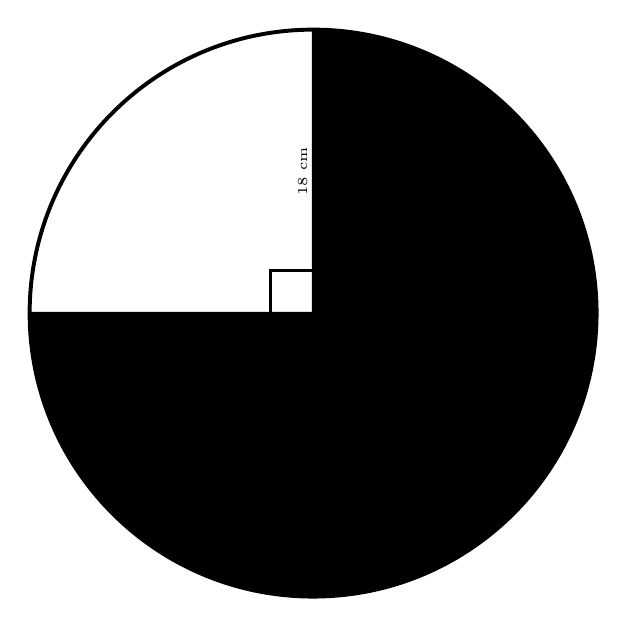
\begin{tikzpicture}[baseline = (current bounding box.west)]


\node[draw, circle, minimum size=2*\radB, inner sep=0pt, line width=0.5mm, outer sep=0] (circ) at (0,0) {};

\node[anchor=south, inner sep=2pt, rotate=90] (18cm.label) at ($(circ.center)!0.5!(90:\radB)$) {\tiny $ \text{18 cm}$};
  
\filldraw[fill=\figurefill, line width=0.3mm]  (90:\radB) arc (90:-180:\radB) -- (circ.center) -- cycle;

\begin{scope} [rotate=90]
\draw[line width=0.3mm] (circ.center) rectangle ++(0.15*\radB,0.15*\radB) node[transform shape]{};
\end{scope} 

\end{tikzpicture} 
 \\
2. 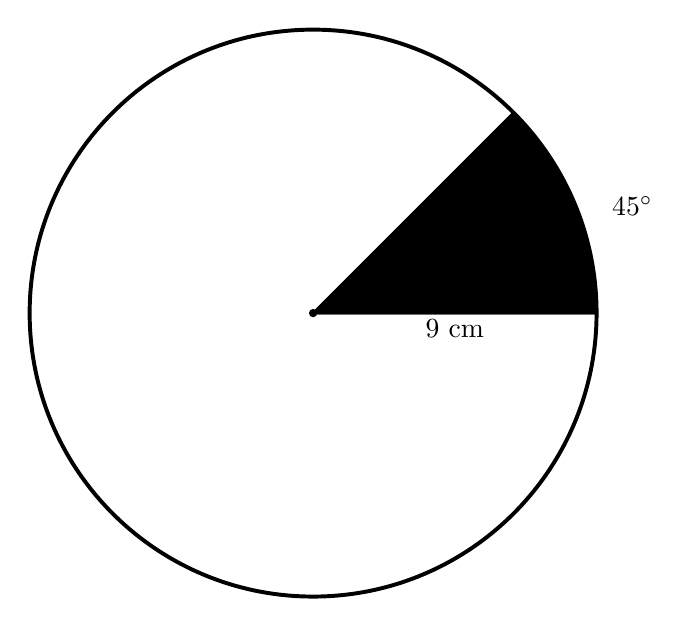
\begin{tikzpicture}[dot/.style={circle, fill=black, inner sep=0pt, outer sep=0pt, minimum size=3pt}, baseline = (current bounding box.west)]

\node[draw, circle, minimum size=2*\radB, inner sep=0pt, line width=0.5mm, outer sep=0] (circ) at (0,0) {};

\node[dot] (circ.dot)  at (circ) {}; 

\coordinate (l) at ($(circ) + (45:\radB)$); 

\coordinate (e) at ($(circ) + (0:\radB)$); 


\draw[line width=0.3mm] (l) -- (circ.center) -- (e);

\node[anchor=north, inner sep=2pt, rotate=0] (9cm.label) at ($(circ.center)!0.5!(e)$) {$ \text{9 cm}$};

\node[anchor=west, inner sep=2pt, rotate=0] (45.label) at (20:1.1*\radB) {$ 45 \degree $};

\filldraw[fill=\figurefill, line width=0.3mm]  (0:\radB) arc (0:45:\radB) -- (circ.center) -- cycle;

\end{tikzpicture}  

 & 6. 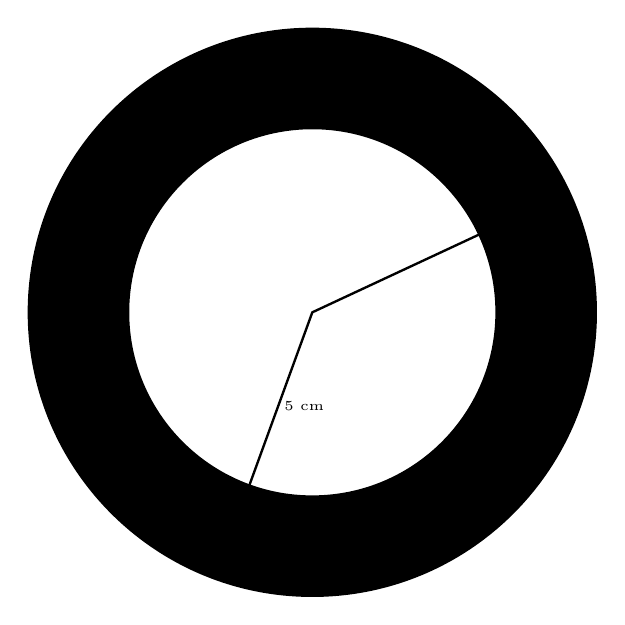
\begin{tikzpicture}[baseline = (current bounding box.west)][dot/.style={circle, fill=black, inner sep=0pt, outer sep=0pt, minimum size=3pt}, dim-label/.style={fill=white, rectangle, inner sep=2pt, outer sep=0pt}%, remember picture, overlay
]  

\coordinate (center) at (0,0);

\filldraw[fill=\figurefill, name path=circ, line width=0.3mm] (center) circle (\radB); 

\filldraw[fill=white, line width=0.3mm] (center) circle (0.65*\radB); 

\node[anchor=west, inner sep=2pt, rotate=0] (5cm.label) at ($(center)!0.35!(250:\radB)$) {\tiny $ \text{5 cm}$};

\node[anchor=west, inner sep=2pt, rotate=0] (3cm.label) at ($(center)!0.87!(250:\radB)$) {\tiny $ \text{3 cm}$};

\draw[line width=0.3mm] (25:0.65*\radB) -- (center) --(250:\radB); 

\end{tikzpicture} 

 \\
3. 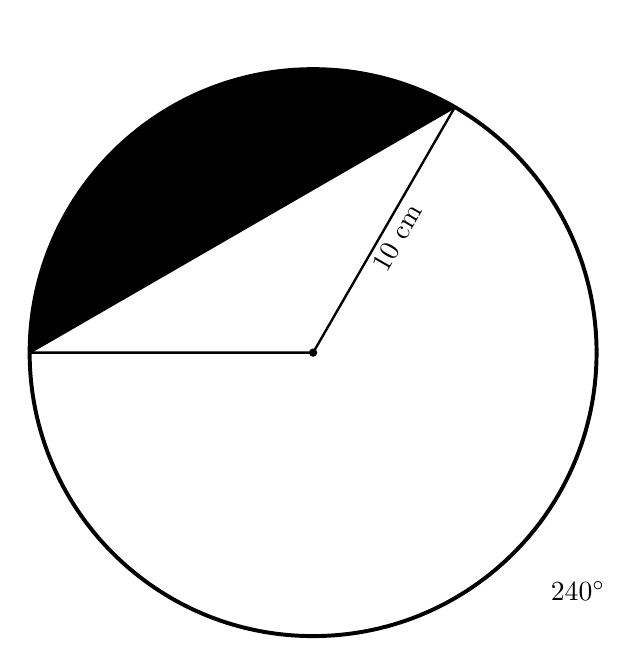
\begin{tikzpicture}[dot/.style={circle, fill=black, inner sep=0pt, outer sep=0pt, minimum size=3pt}, baseline = (current bounding box.west)]

\node[draw, circle, minimum size=2*\radB, inner sep=0pt, line width=0.5mm, outer sep=0] (circ) at (0,0) {};

\node[dot] (circ.dot)  at (circ) {}; 

\coordinate (v) at ($(circ) + (180:\radB)$); 

\coordinate (c) at ($(circ) + (60:\radB)$); 

\draw[line width=0.3mm] (c) -- (circ.center) -- (v) ;

\node[anchor=north, inner sep=2pt, rotate=60] (10cm-label) at ($(circ.center)! 0.5!(c) $)  {$ \text{10 cm}$};  

\node[anchor=north, inner sep=2pt, rotate=0] (240-label) at (-40:1.22*\radB) {$ \text{240\degree } $}; 

\filldraw[fill=\figurefill, line width=0.3mm]  (60:\radB) arc (60:180:\radB) -- cycle;

\end{tikzpicture}  
 & 7. 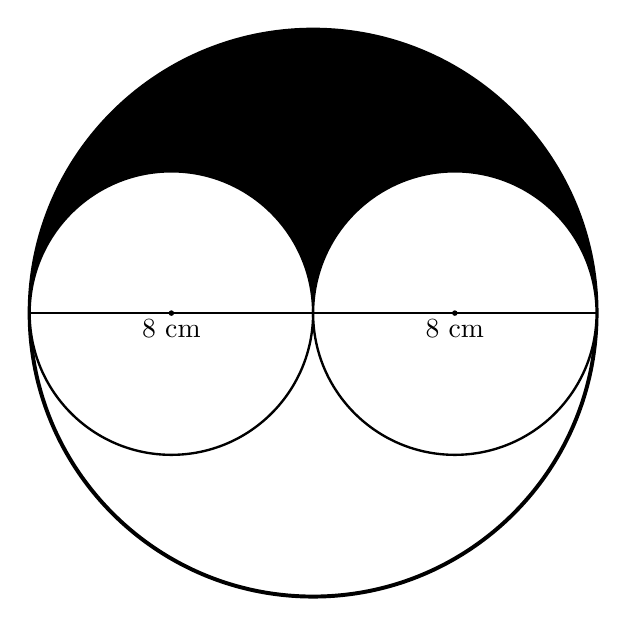
\begin{tikzpicture}[dot/.style={circle, fill=black, inner sep=0pt, outer sep=0pt, minimum size=2pt}, dim-label/.style={fill=white, rectangle, inner sep=2pt, outer sep=0pt}, baseline = (current bounding box.west)]  

\node[draw, circle, minimum size=2*\radB, inner sep=0pt, line width=0.5mm, outer sep=0] (circ) at (0,0) {};

\filldraw[fill=\figurefill, line width=0.3mm]  (180:\radB) arc (180:0:\radB) -- cycle;

\coordinate(center2) at ($(180:\radB)! 0.5! (circ.center) $);

\filldraw[fill=white, line width=0.3mm] (center2) circle (0.5*\radB); 

\coordinate(center3) at ($(0:\radB)! 0.5! (circ.center) $);

\filldraw[fill=white, line width=0.3mm] (center3) circle (0.5*\radB); 

\node [dot] at (center2){}; 

\node [dot] at (center3){}; 


\draw[line width=0.3mm] (180:\radB) -- (0:\radB); 

\node[anchor=north, inner sep=2pt, rotate=0] (8cm1.label) at (center2) {$ \text{8 cm}$};

\node[anchor=north, inner sep=2pt, rotate=0] (8cm2.label) at (center3) {$ \text{8 cm}$};

\end{tikzpicture} 
 \\
4. 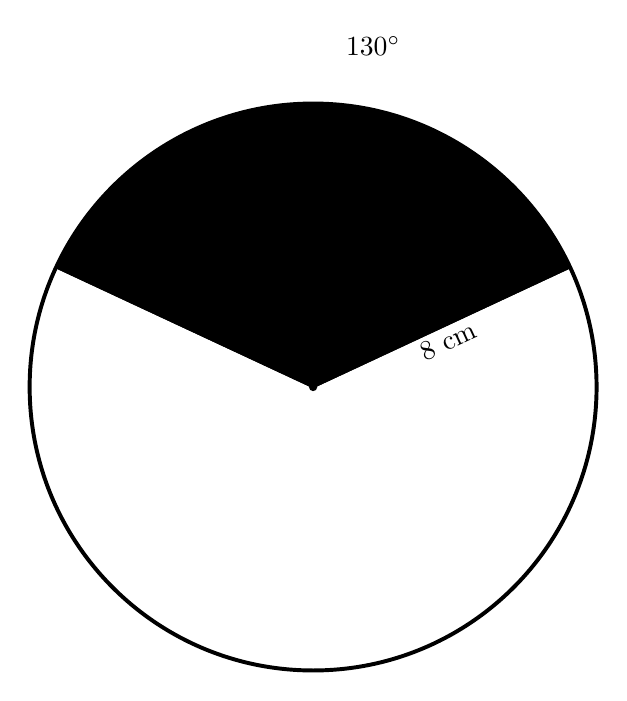
\begin{tikzpicture}[dot/.style={circle, fill=black, inner sep=0pt, outer sep=0pt, minimum size=3pt}, baseline = (current bounding box.west)]

\node[draw, circle, minimum size=2*\radB, inner sep=0pt, line width=0.5mm, outer sep=0] (circ) at (0,0) {};

\node[dot] (circ.dot)  at (circ) {}; 

\coordinate (u) at ($(circ) + (25:\radB)$); 

\coordinate (m) at ($(circ) + (155:\radB)$); 

\draw[line width=0.3mm] (u) -- (circ.center) -- (m) ;

\node[anchor=north, inner sep=2pt, rotate=25] (8cm-label) at ($(u)!0.5!(circ.center)$) {$ \text{8 cm} $};  

\node[rotate=0] (130-label) at ($(circ.center)+(80:1.22*\radB)$) {$ 130\degree $};

\filldraw[fill=\figurefill, line width=0.3mm]  (25:\radB) arc (25:155:\radB) --(circ.center) -- cycle;

\end{tikzpicture}  
 & 8. 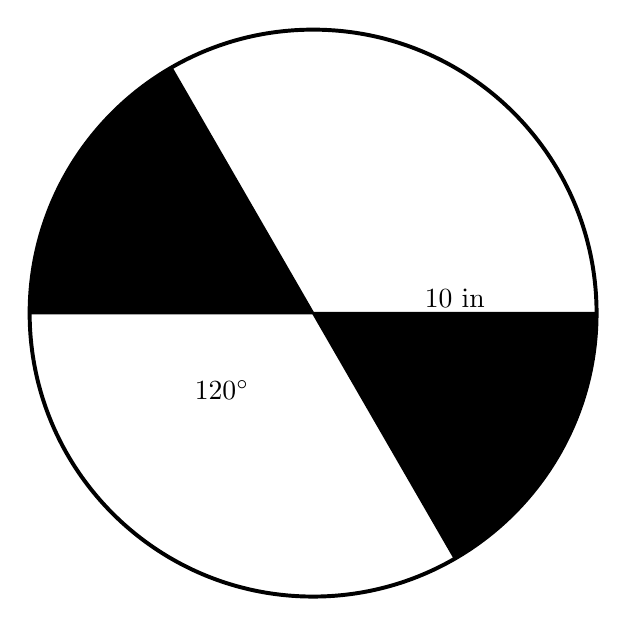
\begin{tikzpicture}[baseline = (current bounding box.west)]



\node[draw, circle, minimum size=2*\radB, inner sep=0pt, line width=0.5mm, outer sep=0] (circ) at (0,0) {};

\node[anchor=south, inner sep=2pt, rotate=0] (10in.label) at ($(circ.center)!0.5!(0:\radB)$) {$ \text{10 in}$};

\filldraw[fill=\figurefill, line width=0.3mm]  (0:\radB) arc (0:-60:\radB) -- (circ.center) -- cycle;

\filldraw[fill=\figurefill, line width=0.3mm]  (180:\radB) arc (180:120:\radB) -- (circ.center) -- cycle;

\node[rotate=0] (120-label) at ($(circ.center)+(220:0.42*\radB)$) {$ 120\degree $}; 


\end{tikzpicture} 

 \\
\end{tabularx}}
\end{minipage}}
\end{center} 
  

}}
\newpage

{\fontsize{36}{40}\fontfamily{pnc}\selectfont {
\input{ps-area-of-sectors-and-segments-of-a-circle-sol}

}}

\end{document}